%%%%%%%%%%%%%%%%%%%%%
%%%%% PREAMBULE %%%%%
%%%%%%%%%%%%%%%%%%%%%
\documentclass[a4paper,12pt,twoside]{book}
\usepackage{fontspec}

%%%%% Index %%%%%
\usepackage{index}
\usepackage{imakeidx}%pour les index, à charger avant hyperref
\makeindex
\makeindex[name=referentiels, title=Index des noms de référentiels]
\makeindex[name=ina, title=Index des termes concernant l'Institut national de l'Audiovisuel]

\usepackage[pdfusetitle, pdfsubject ={Mémoire TNAH}, pdfkeywords={institut national de l'audiovisuel; référentiel; thésaurus; vocabulaire contrôlé; vocabulaire hiérarchique; ontologie; web de données; Wikidata; liens; alignement}]{hyperref}
\usepackage[english, french]{babel}
\usepackage{morewrites}
\usepackage{tocbibind} %paquet pour mettre index et bib dans la toc

% configurer le document selon les normes de l'école
\usepackage[margin=2.5cm]{geometry}
\usepackage{setspace}
\onehalfspacing
\setlength\parindent{1cm}

\usepackage{lettrine}

%%%%% Dessin %%%%%
%\usepackage{qtree}
% avec un code comme ça pour un arbre de classification
%\Tree[.IP [.NP [.Det \textit{the} ]
%[.N\1 [.N \textit{package} ]]]
%[.I\1 [.I \textsc{3sg.Pres} ]
%[.VP [.V\1 [.V \textit{is} ]
%[.AP [.Deg \textit{really} ]
%[.A\1 [.A \textit{simple} ]
%\qroof{\textit{to use}}.CP ]]]]]]
\usepackage{pstricks}
\usepackage{tikz} %paquet pour dessiner ; à placer avant graphicx
\usepackage{graphicx} %paquet image


\usepackage{caption} %pour que la mention de figure n'apparaisse pas dans les légendes de l'image


%%%%% Bibliographie %%%%%
\usepackage[backend=biber, sorting=nyt, style=enc, maxbibnames=3]{biblatex}
\addbibresource{bibliographie/bib.bib}
\nocite{*}
%\defbibnote{intro}{Cette bibliographie contient toutes les références utilisées pour ce cours} %pour des notes introductives dans le début de la biblio

%%%%% Abréviations %%%%%
\usepackage{acro}
\DeclareAcronym{ddcol}{short = DDCOL, long = Direction déléguée aux collections}
\DeclareAcronym{dj}{short = DJ, long = Direction juridique}
\DeclareAcronym{dsi}{short = DSI, long = Direction des systèmes d'information}
\DeclareAcronym{ead}{short = EAD, long = Encoded Archival Description}
\DeclareAcronym{epic}{short = ÉPIC, long = Établissement public à caractère industriel et commercial}
\DeclareAcronym{ina}{short = INA, long = Institut national de l'Audiovisuel}
\DeclareAcronym{isan}{short = ISAN, long = \textit{International Standard Audiovisual Number}}
\DeclareAcronym{lcsh}{short = LCSH, long = Library of Congress Subject Headings}
\DeclareAcronym{marc}{short = MARC, long = MAchine-Readable Cataloging}
\DeclareAcronym{oaipmh}{short = OAI-PMH, long = Open Archive Intiative Protocol for Metadata Harvesting}
\DeclareAcronym{oclc}{short = OCLC, long = Online Computer Library Center}
\DeclareAcronym{ortf}{short = ORTF, long = Office de la radio-télévision française}
\DeclareAcronym{rameau}{short = RAMEAU, long =Répertoire d'autorité-matière encyclopédique et alphabétique unifié}
\DeclareAcronym{unimarc}{short = UNIMARC, long =UNIversal MAchine-Readable Cataloging }


%%%%% Nouvelles commandes %%%%%
\newcommand{\reference}[1]{\autoref{#1}: \nameref{#1}}

\newcommand{\chaptertoc}[1]{\chapter*{#1}
	\addcontentsline{toc}{chapter}{#1}
	\markboth{\slshape\MakeUppercase{#1}}{\slshape\MakeUppercase{#1}}}

\newcommand{\titreEntete}[1]{\markboth{\slshape\MakeUppercase{#1}}{}}

\newcommand{\nP}[2]{#1 \textsc{#2}}

%%%%% Nouveaux environnements %%%%%
\newenvironment{citationLongue}{\begin{quotation}\og}{\fg{}\end{quotation}}

\author{Maxime Challon - M2 TNAH}
\title{Les référentiels en institutions patrimoniales : évolution des pratiques et repositionnement. L’exemple des référentiels de l’Institut national de l’Audiovisuel.}

%%%%%%%%%%%%%%%%%%%%
%%%%% DOCUMENT %%%%%
%%%%%%%%%%%%%%%%%%%%
\begin{document}
	\renewcommand*\appendixautorefname{Annexe}
		
	\frontmatter
	\begin{titlepage}
		\begin{center}
			
			\bigskip
			
			\begin{large}
				\'ECOLE NATIONALE DES CHARTES
			\end{large}
			\begin{center}\rule{2cm}{0.02cm}\end{center}
			
			\bigskip
			\bigskip
			\bigskip
			\begin{Large}
				\textbf{Maxime Challon}\\
			\end{Large}
			\begin{normalsize} \textit{licencié ès histoire}
			\end{normalsize}
			
			\bigskip
			\bigskip
			\bigskip
			
			\begin{Huge}
				\textbf{Les référentiels en institutions patrimoniales : évolution des pratiques et repositionnement}\\
			\end{Huge}
			\bigskip
			\bigskip
			\begin{LARGE}
				\textbf{L’exemple des référentiels de l’Institut National de l’Audiovisuel}\\
			\end{LARGE}
			
			\bigskip
			\bigskip
			\bigskip
			\begin{large}
			\end{large}
			\vfill
			
			\begin{large}
				Mémoire 
				pour le diplôme de master \\
				\og{} Technologies numériques appliquées à l'histoire \fg{} \\
				\bigskip
				2020
			\end{large}
			
		\end{center}
	\end{titlepage}

\thispagestyle{empty}	
\cleardoublepage
	
		\chapter*{Résumé}
	\titreEntete{Résumé}
\addcontentsline{toc}{chapter}{Résumé}
	\medskip
	Ce mémoire, réalisé pour l'obtention du diplôme de Master 2 \og Technologies numériques appliquées à l'histoire\fg{} de l'École nationale des Chartes, retrace l'évolution des pratiques documentaires sur les référentiels en institution patrimoniale à travers l'étude des référentiels de l'\ac{ina} et leurs alignements. Cette étude de l'évolution des formes et des structures des référentiels est liée à l'évolution de la place de ces référentiels au sein des systèmes documentaires, ainsi qu'aux besoins qui leur sont liés.\\
	
	\textbf{Mots-clés~:} institut national de l'audiovisuel; référentiel; thésaurus; vocabulaire contrôlé; vocabulaire hiérarchique; ontologie; web de données; Wikidata; liens; alignement.
	
	\textbf{Informations bibliographiques~:} Maxime Challon, \textit{Les référentiels en institutions patrimoniales : évolution des pratiques et repositionnement. L’exemple des référentiels de l’Institut National de l’Audiovisuel.}, mémoire de master \og{}Technologies numériques appliquées à l'histoire\fg{}, dir. Gautier Poupeau, École nationale des chartes, 2020.
	
		\chapter*{Remerciements}
	\titreEntete{Remerciements}
	\addcontentsline{toc}{chapter}{Remerciements}
	
	\lettrine{M}es remerciements vont tout d'abord à Gautier \textsc{Poupeau}, mon maître de stage, qui m'a accueilli, guidé, conseillé et intégré à son équipe malgré le travail à distance imposé par le contexte actuel. Je souhaite également remercier Axel \textsc{Roche-Dioré} pour ses explications et son soutien dans la réalisation technique de mon stage.\\
	
	J'adresse aussi mes remerciements aux membres du pôle \og Ingénierie de la Donnée\fg{}, Lauryne \textsc{Lemosquet}, Otmane \textsc{Elabboubi} et Akli \textsc{Abdi} pour le temps qu'ils m'ont accordé. \\
	
	Que soit également remercié l'ensemble du département \og Architecture et Innovation\fg{} de l'\ac{ina} pour l'accompagnement fourni tout au long de mon stage, notamment Stanislas \textsc{de Maigret} et Matthieu \textsc{Boricaud} pour le déploiement de l'application, et Olivio \textsc{Ségura} pour la présentation des archives de l'\ac{ina}.
	
	\chaptertoc{Liste des abréviations}
	\printacronyms[heading=none]
	
		\chapter*{\label{introduction_generale}Introduction}
	\titreEntete{Introduction}
\addcontentsline{toc}{chapter}{Introduction}

\begin{citationLongue}
	Toutefois pour ne laisser cette quantité infinie ne la définissant point, [et] aussi pour ne jetter les curieux hors d'espérance et pouvoir acco[m]plir [et] venir à bout de cette belle entreprise, il me semble qu'il est à propos de faire comme les Médecins, qui ordonnent la quantité des drogues suivant la qualité d'icelles, [et] de dire que l'on ne peut manquer de recueillir tous ceux qui auront les qualitez [et] conditions requises pour estre mis dans une Bibliotheque.\footcite[p.41-42]{naude_advis_1627}
\end{citationLongue}


\lettrine{E}n 1627, \nP{Gabriel}{Naudé} compare le médecin au bibliothécaire, semblables par leur nécessité d'ordonner pour sélectionner, de classer pour retrouver, au milieu d'une masse d'objets. Cet ordonnancement, ce classement, passent pas une hiérarchisation de leur connaissance ou de leurs outils, dans le but de faciliter la recherche d'un médicament ou d'un livre pour l'utilisateur final. Cependant, plusieurs siècles plus tard, la hiérarchisation de la connaissance, ayant pour but de référencer une instance de la vie réelle, ne fonctionne plus: l'utilisateur ne part plus que très rarement d'un terme de la hiérarchie pour trouver son document; il utilise le plus souvent un mot ou un concept qui le renverront vers une liste de résultats correspondant à sa requête. Alors, la notion de graphe prend le dessus sur celle de hiérarchie.\\

La notion évoquée de \og quantité infinie \fg{} est aujourd'hui d'autant plus valable avec le web et l'explosion des quantités de données produites et stockées: avec cette mort de la notion de ressource, et par conséquent de celle de référentiel, la donnée structurée est implantée, peut être exploitée à la fois par une machine et par une personne, et est divisible et modulable à l'infini.\\

Cette transition de la ressource à la donnée, des référentiels hiérarchiques aux référentiels en graphe, est observable à l'\ac{ina}. Créé en 1975 suite au démantèlement en sept sociétés de l'\ac{ortf} par la loi du 07 août 1974, l'\ac{ina} est désigné comme un \ac{epic} et \og chargé de la conservation des archives, des recherches de créations audiovisuelles et de la formation professionnelle\fg{}\footcite[art.3]{noauthor_loi_1974}. À ces missions est ajouté à partir de 1992 le dépôt légal de la télévision, de la radio, de la télévision satellite, par câble et numérique. Cette massification continue de documents et de données nécessite un classement et un référencement efficace des collections, ce qui a conduit à la création de plusieurs référentiels dans l'Institut.\\

Face à la croissance de l'utilisation du numérique, à l'accroissement des collections et des données à l'\ac{ina} depuis les numérisations des collections au début des années 2000, aux nouveaux besoins exprimés par les professionnels et le public, une refonte du système documentaire est mise en place à la \ac{dsi} au sein du département \og Architecture et Innovation\fg{}: les données et leurs métadonnées sont extraites des anciens silos de conservation, puis transformées et migrées dans un nouveau système d'information centralisé. Ainsi, les référentiels, descripteurs de chaque document, identificateurs de personnes ou d'instances des collections, subissent également ce traitement pour les uniformiser et permettre une homogénéisation et une meilleure valorisation des données de l'\ac{ina}.\\

Cette migration massive permet d'observer l'évolution des pratiques documentaires de référencement et de description de ces dernières décennies, suivant la même évolution que l'ensemble du milieu bibliothéconomique en France, ainsi que les changements de structure des référentiels utilisés. La diversité de formes et de structures des référentiels montre que ces derniers sont considérés seulement comme des outils à disposition du documentaliste pour décrire ses fonds; périphériques et éclatés, ils ne permettent pas une centralisation uniforme des données de l'\ac{ina}.\\

Le projet du \textit{Lac de données}, débuté en 2014, a pour but de centraliser l'ensemble des données de l'\ac{ina}, les référentiels prenant alors une place centrale dans le nouveau système d'information. Ce projet s'inscrit dans l'évolution des besoins, tant chez les documentalistes que chez les utilisateurs, avec une utilisation désormais massive du web par tous les publics - chercheurs, professionnels des médias, jeunesse, \dots - pour la recherche et la consultation de contenus. Cette éditorialisation croissante et indispensable nécessite de nombreuses données de référence, par lesquelles les contenus sont cherchables et trouvables.\\

Ce mémoire offre une réflexion sur ces évolutions des pratiques et des usages des référentiels à l'\ac{ina}, et plus généralement dans une institution patrimoniale. Au-delà de ces évolutions sensibles, c'est le positionnement du référentiel au sein des systèmes documentaires qu'il est nécessaire d'interroger, de manière à faire face aux nouveaux enjeux et aux nouveaux besoins exprimés ces dernières années: d'un rôle périphérique, pensé comme un outil, le référentiel devient désormais un pivot autour duquel les données documentaires se raccrochent.\\

Mon stage, débuté en mai 2020 et terminé fin août 2020, à la \ac{dsi} de l'\ac{ina}, m'a permis d'intégrr le département \og Architecture et Innovation\fg{} de \nP{Gautier}{Poupeau}, et plus particulièrement le pôle \og Ingénierie de la Donnée\fg{} dirigé par \nP{Axel}{Roche-Dioré}, afin d'effectuer une réflexion sur les méthodes d'alignement de plusieurs référentiels, et de mettre en œuvre ces méthodes. Les échanges avec mes collègues du pôle \og Ingénierie de la Donnée\fg{} et les professionnels de la documentation de la \ac{ddcol} et de la \ac{dj} m'ont permis de naviguer dans les référentiels, d'observer leurs différences, leurs structures, de comprendre les besoins qui leurs étaient associés ainsi que les difficultés impliquées par chaque référentiel dans l'opération d'alignement en vue de leur migration vers le \textit{Lac de données}. Plusieurs missions m'ont ainsi été confiées:
\begin{itemize}
	\item Extraire les fonctions et les occupations de personnes physiques depuis les notes qualité en texte libre du référentiel des personnes physiques et morales de la \ac{ddcol}, puis aligner ces fonctions extraites avec un thésaurus de noms communs propre à la \ac{ddcol}
	\item Aligner les personnes physiques de la \ac{ddcol} avec les entités correspondantes de \href{https://www.wikidata.org/}{Wikidata}
	\item Aligner les fictions et les séries conservées à l'\ac{ina} avec \href{https://www.wikidata.org/}{Wikidata} de manière à récupérer également l'identifiant \ac{isan}
	\item Aligner les référentiels de personnes physiques de la \ac{dj} et de la \ac{ddcol}, puis développer une interface de vérification et de complétion des alignements réalisés automatiquement
\end{itemize}
\bigskip

Ce mémoire retrace l'évolution des usages et des pratiques documentaires concernant les référentiels dans les institutions patrimoniales, en s'appuyant sur l'exemple des référentiels de l'\ac{ina}. Dans un premier temps, dans une période allant jusqu'au début des années 2000, les référentiels sont uniquement considérés comme des fournisseurs de clés entre les données de manière à les contrôler plus facilement. Puis, jusqu'au milieu des années 2010, le web et le web de données permettent une mise en commun des référentiels qui se retrouvent alors liés entre eux. Enfin, depuis le milieu des années 2010, les référentiels sont placés au centre des systèmes d'information: ils sont devenus les pivots des systèmes documentaires.


\thispagestyle{empty}
\cleardoublepage
	
	\mainmatter
	
	\part{\label{controler}CONTRÔLER. A la recherche de clés (années 1960 – fin des années 1990)}
	
	\chapter{\label{I-A}Le référentiel comme clé}
\titreEntete{Le référentiel comme clé}

\lettrine{C}onsidéré comme une simple aide ou outil au service du documentaliste ou de l'utilisateur, le référentiel trouve d'abord sa place comme fournisseur de clés. Son utilisation principale est d'offrir au document décrit des vedettes qui puissent permettre une classification ou une recherche aisée de ce document. Cependant, pour être efficaces, ces vedettes doivent partager un langage contrôlé, des règles de graphie, de syntaxe, \dots~ D'abord conservées sur des fichiers papier en institutions patrimoniales, ces vedettes ont été parmi les premiers éléments rétroconvertis, donnant naissance aux fichiers d'autorité numériques, et permettant une interopérabilité entre les référentiels par le biais des portails numériques.

\section{\label{I-A-1}Du langage libre au langage contrôlé: vers l'indexation}

\section{\label{I-A-2}Une clé entre les données: les vocabulaires contrôlés}
\titreEntete{Une clé entre les données}

Dans les \index[ref]{typologie@Typologie!vocabulaires controles@Vocabulaires contrôlés}vocabulaires contrôlés, les termes servant à la description sont soumis à une normalisation. La maîtrise de la terminologie est l'objectif de ces vocabulaires et ce qui permet à ces derniers d'être une \og colle qui tient l'ensemble du système \footnote{\og Controlled vocabularies have become the glue that holds the system together \fg{} in \cite{rosenfeld_information_2015}}\fg{} pour le rendre cohérent. Ces vocabulaires ne sont pas hiérarchisés et tirent la description de leur terme uniquement par leur graphie et leur désambiguïsation face au langage naturel. Ils permettent d'éviter les erreurs de graphie introduites par le documentaliste --- par conséquent les différences de graphies --- , d'éviter également les redondances de termes similaires et de rendre un système univoque.
Ainsi, les vocabulaires contrôlés deviennent à eux seuls des langages propres à leurs utilisateurs\footnote{Le Centre National de Ressources Textuelles et Lexicales \href{https://www.cnrtl.fr/definition/vocabulaire}{(CNRTL)} définit ainsi un vocabulaire: \og Dictionnaire ne comportant que les mots les plus usuels d'une langue\fg{}}, servant à lutter contre la trop grande richesse du langage naturel humain.
Pour effectuer le contrôle des termes, plusieurs points de contrôle sont introduits: le contrôle de la forme des vedettes, celui de la polysémie et celui de la synonymie. L'exemple des autorités \index[ref]{lod@Linked Open Data (LOD)!rameau@RAMEAU}\index[ref]{autorites@Autorités!rameau@RAMEAU}\ac{rameau}\footcite{bibliotheque_nationale_de_france_rameau_nodate} et des \index[ref]{lod@Linked Open Data (LOD)!lcsh@LCSH}\index[ref]{autorites@Autorités!lcsh@LCSH}\ac{lcsh}\footcite{the_library_of_congress_library_nodate}, bien que comprenant une hiérarchie et des relations complexes, permettent d'observer la formation d'un langage contrôlé.

\subsection{\label{I-A-2-a}Contrôle de la forme des vedettes}
\titreEntete{Contrôle de la forme des vedettes}

La forme des vedettes doit être contrôlée de manière à offrir une graphie uniformisée; plusieurs moyens sont alors utilisés:
\begin{itemize}
	\item Choix d'un mot ou d'une locution en langage libre, le plus général possible, en évitant les ambiguïtés: le \index[ref]{lod@Linked Open Data (LOD)!rameau@RAMEAU}\index[ref]{autorites@Autorités!rameau@RAMEAU}\ac{rameau} a fait le choix de \og \href{https://data.bnf.fr/fr/11933646/television}{Télévision}\fg{}, de même que les \index[ref]{lod@Linked Open Data (LOD)!lcsh@LCSH}\index[ref]{autorites@Autorités!lcsh@LCSH}\href{http://id.loc.gov/authorities/subjects/sh85133456.html}{\ac{lcsh}}
	\item Utilisation d'une langue définie pour l'ensemble du vocabulaire, sauf pour le cas d'emprunts: \ac{rameau} est en français, on y trouve alors la vedette \og \href{https://data.bnf.fr/fr/13318464/droit_d_auteur/}{Droit d'auteur}\fg{} au lieu de \og Copyright\fg{}, alors que les vedettes \ac{lcsh} considèrent l'inverse: \og\href{http://id.loc.gov/authorities/subjects/sh85032446.html}{Copyright} \fg{} avec une variante en français renvoyant vers la vedette \ac{rameau}. Cependant, des variantes linguistiques sont attachées aux vedettes: l'italien \og Televisione\fg{} est ainsi lié à la vedette \og \href{https://data.bnf.fr/fr/11933646/television}{Télévision}\fg{} de \ac{rameau}
	\item Utilisation majoritaire du pluriel pour les noms communs (comme la vedette \ac{rameau} \og \href{https://data.bnf.fr/fr/11932295/livres/}{Livre \fg{}}); le singulier étant utilisé pour les concepts généraux (\og \href{https://data.bnf.fr/fr/11936326/ecriture/}{Écriture}\fg{})
	\item Choix d'une forme plus attestée ou plus usitée qu'une autre: nous pouvons trouver \og \href{https://data.bnf.fr/fr/11960499/radiodiffusion/}{Radiodiffusion}\fg{} et non \og Radio\fg{} dans \index[ref]{lod@Linked Open Data (LOD)!rameau@RAMEAU}\index[ref]{autorites@Autorités!rameau@RAMEAU}\ac{rameau}; de même, nous constatons la présence de \og \href{http://id.loc.gov/authorities/subjects/sh85110448.html}{Radio broadcasting}\fg{} dans \index[ref]{lod@Linked Open Data (LOD)!lcsh@LCSH}\index[ref]{autorites@Autorités!lcsh@LCSH}\ac{lcsh}, la vedette \og \href{http://id.loc.gov/authorities/subjects/sh85110385.html}{Radio}\fg{} étant réservée pour le moyen de communication
\end{itemize}

\subsection{\label{I-A-2-b}Contrôle de la polysémie et de l'homographie}
\titreEntete{Contrôle de la polysémie et de l'homographie}

L'ambiguïté du langage naturel dans la graphie et la polysémie peut induire le documentaliste et l'utilisateur en erreur, et réduire ainsi la puissance et l'utilité du vocabulaire mis en place. Contrôler la polysémie et l'homographie est, par conséquent, indispensable. Une vedette doit alors correspondre à un seul concept: deux actions sont alors possibles pour supprimer les ambiguïtés et améliorer le vocabulaire.
\begin{itemize}
	\item L'ajout d'un qualificatif entre parenthèses peut permettre la levée de cette ambiguïté: \index[ref]{lod@Linked Open Data (LOD)!rameau@RAMEAU}\index[ref]{autorites@Autorités!rameau@RAMEAU}\ac{rameau} utilise les qualificatifs \og \href{https://data.bnf.fr/fr/11935557/iris__plantes_/}{Plantes}\fg{} et \og\href{https://data.bnf.fr/fr/11938389/iris__anatomie_/}{Anatomie}\fg{} pour traiter l'homonymie de \og Iris\fg{}; cette ambiguïté existant également en anglais, \index[ref]{lod@Linked Open Data (LOD)!lcsh@LCSH}\index[ref]{autorites@Autorités!lcsh@LCSH}\ac{lcsh} utilise les mêmes qualificatifs (\og \href{https://id.loc.gov/authorities/subjects/sh85068079.html}{Plants}\fg{} et \og\href{https://id.loc.gov/authorities/subjects/sh85068076.html}{Eye}\fg{})
	\item L'utilisation de l'opposition singulier/pluriel permet de distinguer un concept abstrait d'une réalité concrète: \index[ref]{lod@Linked Open Data (LOD)!rameau@RAMEAU}\index[ref]{autorites@Autorités!rameau@RAMEAU}\ac{rameau} utilise cette opposition de genre pour séparer le \og \href{https://data.bnf.fr/fr/11936118/cinema/}{Cinéma}\fg{} compris comme art, du \og \href{https://data.bnf.fr/fr/11939426/cinemas/}{cinéma}\fg{} compris comme bâtiment où cet art est projeté
\end{itemize}

\subsection{\label{I-A-2-c}Contrôle de la synonymie}
\titreEntete{Contrôle de la synonymie}

Le dernier écueil des vocabulaires contrôlés est la synonymie: source de confusions, elle conduit à la création de nombreuses vedettes qui se rapportent finalement à un même concept. \index[ref]{lod@Linked Open Data (LOD)!lcsh@LCSH}\index[ref]{autorites@Autorités!lcsh@LCSH}\ac{lcsh} et \index[ref]{lod@Linked Open Data (LOD)!rameau@RAMEAU}\index[ref]{autorites@Autorités!rameau@RAMEAU}\ac{rameau} ont fait le choix de créer des termes exclus qui renvoient vers le concept auquel ils sont reliés: ainsi, une recherche du terme \og \href{https://data.bnf.fr/fr/search?term=detenus#Rameau}{Détenus}\fg ~dans \ac{rameau} renvoie vers la vedette \og\href{https://data.bnf.fr/fr/13318775/prisonniers/}{Prisonniers}\fg{}. Les termes exclus peuvent être de différents types:
\begin{itemize}
	\item des synonymes: \og Cameramen \fg{}, \og Cinematographers\fg{}, \og Operating Cameraman\fg{} sont tous des termes exclus et synonymes de \og\href{https://id.loc.gov/authorities/subjects/sh2002011142.html}{Cameraman}\fg{} dans les \ac{lcsh}
	\item des abréviations ou des acronymes: l'abréviation \og ISSN\fg{} est ainsi un terme exclu de l'\og\href{https://id.loc.gov/authorities/subjects/sh85067450.html}{\textit{International Standard Serial Numbers}}\fg{} dans les \ac{lcsh}
	\item des inversions de termes --- qui permettent la mise en avant d'un terme important --- : \index[ref]{lod@Linked Open Data (LOD)!lcsh@LCSH}\index[ref]{autorites@Autorités!lcsh@LCSH}\ac{lcsh} considère comme terme exclu de \og\href{https://id.loc.gov/authorities/subjects/sh2002011142.html}{Cameraman}\fg{} \og Operators, Camera\fg{}
	\item enfin, les termes exclus peuvent être des constructions syntaxiques, permettant de supprimer l'ambiguïté encore présente ou alors de préciser le champ de la vedette: \ac{rameau} précise ainsi l'étendue géographique des vedettes en ajoutant le nom du pays après le concept; la nouvelle vedette ainsi créée devient restrictive et spécifique. C'est le cas notamment de \og\href{https://data.bnf.fr/fr/11979998/chaines_de_television_--_france/}{Chaînes de télévision -- France}\fg{} qui précise la vedette \og\href{https://data.bnf.fr/fr/11936935/chaines_de_television/}{Chaînes de télévision}\fg{} dans \index[ref]{lod@Linked Open Data (LOD)!rameau@RAMEAU}\index[ref]{autorites@Autorités!rameau@RAMEAU}\ac{rameau}.
\end{itemize}
\bigskip
\bigskip

\begin{figure}[!h]
	\centering
\begin{pspicture}(0,1)(9,9)	
	\psdot(5,8)
	\uput[0](3.7,8.5){\textsc{Prisonniers}}	
	\psdot(5,2)
	\uput[-180](6,1.5){Bagnards}	
	\psdot(8,5)
	\uput[0](8.1,5){Détenus}	
	\psdot(2,5)
	\uput[0](0,5){Forçats}	
	\psdot(2.9,2.9)
	\uput[0](0.6,2.9){Galériens}
	\psdot(7.1,2.9)
	\uput[0](7.5,2.9){Personnes détenues}
	\psdot(2.9,7.1)
	\uput[0](-2,7.1){Personnes incarcerées}
	\psdot(7.1,7.1)
	\uput[0](7.3,7.1){Population carcérale}
	
	\uput[0](3,5){\textbf{Vedette \href{https://data.bnf.fr/fr/13318775/prisonniers/}{Prisonniers}}}
	
	\pscircle(5,5){3}
\end{pspicture}
\caption{Anneau de synonymie du terme \og \href{https://data.bnf.fr/fr/13318775/prisonniers/}{Prisonniers}\fg{} de \ac{rameau}}
\label{synonym_ring_rameau}
\end{figure}
\begin{figure}[!h]
	\centering
\begin{pspicture}(0,1)(9,9)
	\psdot(5,8)
	\uput[0](3.7,8.5){\textsc{Prisoners}}	
	\psdot(5,2)
	\uput[-180](6,1.5){Convicts}	
	\psdot(2.4,6.5)
	\uput[0](-1.8,6.5){Incarcerated persons}	
	\psdot(7.6,3.6)
	\uput[0](7.8,3.6){Prison inmates}	
	\psdot(2.4,3.6)
	\uput[0](-1.8,3.6){Imprisoned persons}
	\psdot(7.6,6.5)
	\uput[0](7.8,6.5){Correctional institutions--Inmates}
	
	\uput[0](3,5){\textbf{Vedette \href{https://id.loc.gov/authorities/subjects/sh85106950.html}{Prisoners}}}
	
	\pscircle(5,5){3}
\end{pspicture}
\caption{Anneau de synonymie du terme \og \href{https://id.loc.gov/authorities/subjects/sh85106950.html}{Prisoners}\fg{} de \ac{lcsh}}
\label{synonym_ring_lcsh}
\end{figure}

 Ces termes exclus permettent de multiplier les points d'accès à un concept en prenant en compte la complexité du langage naturel qui désigne souvent par différents termes un même concept. Ainsi, deux utilisateurs cherchant la même vedette mais avec des termes différents pourront plus facilement retrouver cette vedette. Si ces termes ne sont pas obligatoirement des synonymes, leur contexte et le vocabulaire dans lesquels ils se trouvent les font se considérer comme synonymes\footcite{rosenfeld_information_2015}. \nP{Peter}{Morville} et \nP{Louis}{Rosenfeld} nomment ces rapprochements des \og Anneaux de synonymie\fg{}\footnote{\og Synonym rings\fg{} in \cite{rosenfeld_information_2015}. Voir \reference{synonym_ring_rameau} et \reference{synonym_ring_lcsh}.}: ils connectent un ensemble de mots qui sont compris comme équivalents dans leur contexte d'utilisation\footnote{\og Connects a set of words that are defined as equivalent for the purposes of the retrieval.\fg{} in \cite{rosenfeld_information_2015}}.

\section{\label{I-A-3}Une clé entre les jeux de données: l'interopérabilité par les fichiers d'autorité et les portails}
\titreEntete{Une clé entre les jeux de données}

Comme nous l'avons évoqué précédemment (voir \reference{I-A-2}), les vocabulaires contrôlés sont de nouveaux langages, spécifiques et uniformisés, se substituant au langage naturel humain pour un domaine précis. Le vocabulaire est par conséquent un référentiel propre à l'institution qui l'a créée et a pour seul utilisateur cette institution. Seulement, deux institutions aux activités proches créent deux vocabulaires similaires, se distinguant par la complétude de certaines vedettes ou par des variantes de graphies.\\
Le domaine bibliothéconomique a été le premier à informatisé ses vocabulaires et ses fichiers d'autorités en masse, permettant ainsi une amélioration de l'expérience utilisateur et du catalogage, et un partage possible avec des institutions proches.

\subsection{\label{I-A-3-a}La naissance des autorités par rétroconversion}
\titreEntete{Les fichiers d'autorité}

\begin{citationLongue}
	Les fichiers d'autorité appartiennent bien à un	ensemble : fonctionnant comme un tout, avec des règles d’interdépendance et d’interopérabilité de ses constituants, ils permettent le contrôle de	la cohérence des métadonnées bibliographiques.\footcite[p.6]{aymonin_arabesques_2017}
\end{citationLongue}

Avant la naissance du web, chaque ouvrage était décrit dans un catalogue et classé par ordre alphabétique des noms d'auteur. Des catalogues thématiques ont été créés, de même que des fichiers physiques en bibliothèque, permettant la recherche de documents selon un sujet précis. Cependant, l'indexation des documents est réduite au titre, à l'auteur, et à quelques sujets. En effet, la structure même d'un fichier papier en bibliothèque nécessite de dupliquer la notice d'un exemplaire en plusieurs notices qui vont être placées par la suite dans le fichier correspondant au sujet.\\

Ces fichiers physiques des bibliothèques, bien qu'utiles aux lecteurs par leur classement thématique, présentent plusieurs difficultés: d'abord, l'indexation se trouve limitée à quelques mots; ensuite, la création d'un fichier thématique est complexe à réaliser par le choix des vedettes et produit alors un immense silence; enfin, la consultation d'une fiche par un lecteur empêche un second de la consulter dans le même temps.\\

Dès les années 1970, les bibliothèques se sont engagées dans une vaste opération de rétroconversion de leurs notices documentaires. Les fichiers physiques et les notice cartonnées sont alors informatisés et \og reproduits presque à l’identique [\dots] sous forme de bases de données\fg{}\footcite{bermes_1_2013}. L'informatisation des notices et des fichiers permet par conséquent d'améliorer l'indexation des documents, et à l'utilisateur de pouvoir trouver plus de documents correspondant à sa recherche plus rapidement. Ainsi, les autorités \ac{lcsh}, créées en 1914 sous format papier, ont été informatisées; les autorités \ac{rameau} créées dans les années 1980 reprennent celles \ac{lcsh} en les complétant.\\

Cependant, ces fichiers d'autorité comportent, comme nous l'avons évoqué plus haut (\reference{I-A-2-c}), des formes retenues et des formes rejetées des termes, ce qui créé de multiples renvois à l'intérieur du fichier physique ou informatique. L'arrivée des moteurs de recherche dans les années 2000 permet de supprimer ces différences de termes en indexant à la fois les formes retenues et les formes rejetées, permettant de trouver directement la vedette recherchée.

\subsection{\label{I-A-3-b}Partager des vocabulaires: à la recherche de la meilleure interopérabilité}
\titreEntete{Partager des vocabulaires}

La problématique du partage des référentiels entre institutions se pose avant l'informatisation des catalogues et des fichiers des bibliothèques. En effet, le format \ac{marc}, né en 1968 à la Bibliothèque du Congrès, permet l'échange de données entre les institutions et la \og duplication les notices d’un catalogue à un autre\fg{}\footcite{bermes_2_2013}. Malgré de multiples variantes nationales, l'\ac{unimarc} reste aujourd'hui le format d'échange privilégié entre les bibliothèques.\\

Pour partager les fichiers d'autorité et aboutir à une interopérabilité totale des données entre deux institutions par le biais des machines, différents protocoles d'échange ont été utilisés --- ou délaissés en fonction des difficultés imposées par chacun---. Dès les années 1980 est développé le protocole Z39-50. Ce protocole permet d'interroger une base de données de manière synchrone, selon la requête du client, et de récupérer des données en format \ac{marc}\footcite{bibliotheque_nationale_de_france_protocole_nodate}.\\

Ce protocole Z39-50 est destiné aux catalogueurs qui peuvent ainsi \og repérer puis télécharger une notice dans un catalogue distant plutôt que d’avoir à la saisir \textit{ex nihilo}\fg{}\footcite{bermes_2_2013}. Le partage, \og par conversion et copie\fg{}\footnote{\cite{bermes_2_2013}. Voir \reference{annexe_types_interop}}, n'est alors qu'une simple copie de données, dont la mise à jour est difficile. L'existence de ce protocole, bien que destiné aux professionnels de la documentation, a suscité la création de portails de consultation de notices documentaires ou de fichiers d'autorité, interrogeant de manière synchrone les bases de données: cette utilisation orientée utilisateur du protocole Z39-50 permet à la Bibliothèque nationale de France d'offrir différents services(intégration des notices dans \ac{oclc}, recherche dans le Catalogue Collectif de France (CCFR), \dots\footcite{bibliotheque_nationale_de_france_protocole_nodate}). Cependant, face aux temps de réponses importants et aux résultats appauvris retournés par la requête, les portails se sont révélés décevants et peu efficaces. De plus, l'utilisation d'un portail nécessite de la part de l'utilisateur qu'il connaisse précisément ce qu'il cherche de manière à se connecter au portail correspondant (sui lui-même doit être connu de cet utilisateur)\footcite{dalbin_approches_2011}.\\

La multiplication des formats d'échanges --- \ac{marc} et \ac{unimarc} pour les bibliothèques, \ac{ead} pour les archives ---, ainsi que la volonté d'offrir au public lien entre les différentes bases de données patrimoniales, ont conduit à la création d'un nouveau protocole, \ac{oaipmh}. Ce protocole asynchrone repose sur deux acteurs: le fournisseur qui met à disposition ses données dans un \og entrepôt\fg{}, et le moissonneur qui collecte ces données pour les intégrer à son système\footcite{bibliotheque_nationale_de_france_protocole_nodate-1}.\\

Cependant, si les performances du protocole sont améliorées avec \ac{oaipmh}, les documents et les fichiers d'autorité ne peuvent pas être sélectionnés et filtrés: un format d'échange simple, minimal, est nécessaire. Ce format est le Dublin Core\footcite{noauthor_dublin_nodate} comprenant quinze champs d'informations.
Ce partage de données et de métadonnées entre les institutions permet une \og interopérabilité par le plus petit dénominateur commun\fg{}\footnote{\cite{bermes_2_2013}. Voir \reference{annexe_types_interop}}, où ce dénominateur est le Dublin Core. Ce dénominteur commun peut néanmoins présenter un appauvrissement des données puisque les champs sont très réduits, ou au contraire permettre de grandes différences au sein d'un même champ.

\bigskip
\bigskip
\bigskip
Auteurs, catalogueurs et bibliothécaires ont très vite ressenti le besoin de se dégager du langage naturel de manière à renvoyer rapidement vers des passages de leur texte ainsi qu'à décrire le plus précisément possible les documents, pour faciliter la lecture ou la recherche de l'utilisateur final. D'abord effectuées sur des supports papier, ces opérations de descriptions ont été informatisées et ont permis le partage de données et de métadonnées entre les institutions: les notices et les fichiers d'autorité disponibles sont la source constante d'interrogations quant au meilleur moyen de les mettre à disposition, tant pour le professionnel que pour le public. L'ouverture de ces vocabulaires a permis une amélioration des descriptions et une uniformisation des pratiques d'indexation.\\

Cependant, ces vocabulaires contrôlés restent peu précis et sont limités à leur terminologie pour en tirer le sens: il ne comprennent pas de terminologie sémantique, qui permettrait alors d'améliorer davantage la description effectuée, en se référerant aux termes parents, frères ou fils. L'anneau de synonymie évoqué (\reference{I-A-2-b}) permet la prise en compte des synonymes, mais ne donne pas de sens supplémentaire à la vedette.
	\chapter{\label{I-B}Les référentiels à l’INA}
\titreEntete{Les référentiels à l’INA}
	\chapter{\label{I-C}Les référentiels à l’INA}
	\titreEntete{Les référentiels à l’INA}
	
	\part{\label{relier}RELIER. Vers le partage de référentiels communs (début des années 2000 – milieu des années 2010)}
	
	\chapter{\label{II-A}Le web de données: une exposition commune des référentiels}
	\titreEntete{Le web de données: une exposition commune des référentiels}
	\chapter{\label{II-B}Partager des structurations similaires de jeux de données par les classes et les propriétés : les ontologies, grammaires communes mais spécifiques}
	\titreEntete{Les ontologies, grammaires communes mais spécifiques}
	\chapter{\label{II-C}Relier ses données à Wikidata}
	\titreEntete{Relier ses données à Wikidata}
	
	\part{\label{centraliser}CENTRALISER. Le référentiel, clé de voûte et pivot (depuis le milieu des années 2010)}	
	
	\chapter{\label{III-A}Les labyrinthes comme réseaux de données et de liens}
	\titreEntete{Les labyrinthes comme réseaux de données et de liens}
	\chapter{\label{III-B}Le Lac de données de l’INA : le référentiel au centre du modèle}
	\titreEntete{Le référentiel au centre du modèle}
	\chapter{\label{III-C}Centraliser les référentiels de l’INA dans le Lac de données: l'exemple de l'alignement de deux référentiels de personnes physiques}
	\titreEntete{Aligner deux référentiels de personnes physiques}

	\chaptertoc{Conclusion}
\titreEntete{Conclusion}

%historique de struct ref: arbre au laby et modele reseau

%changement des usages et des besoins...

%... qui produit changement place ref
	
	\appendix
	\part*{Annexes}	
	\addcontentsline{toc}{part}{Annexes}
	\setcounter{chapter}{0}

\chapter{\label{annexe_index_schoepflin}Les index de la Renaissance, termes contrôlés et classification alphabétique (les index de l'\textit{Alsatia Illustrata} de \nP{Jean-Daniel}{Schoepflin})}
\titreEntete{Annexe \thechapter}

\begin{figure}[!h]
	\centering
	\begin{minipage}[c]{.46\linewidth}
		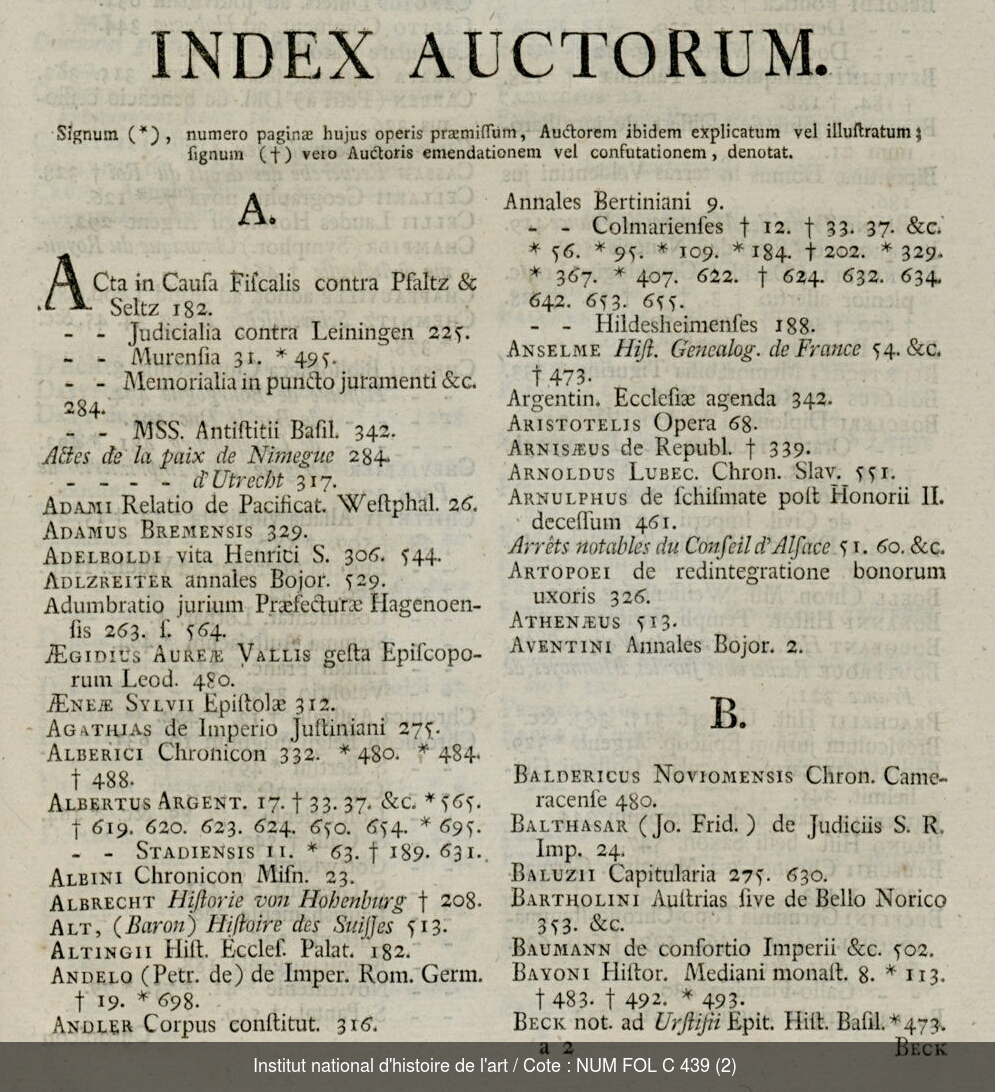
\includegraphics[width=6cm]{images/index_auctorum_alsatia.jpg}
		\caption{Index auctorum}
	\end{minipage} \hfill
	\begin{minipage}[c]{.46\linewidth}
		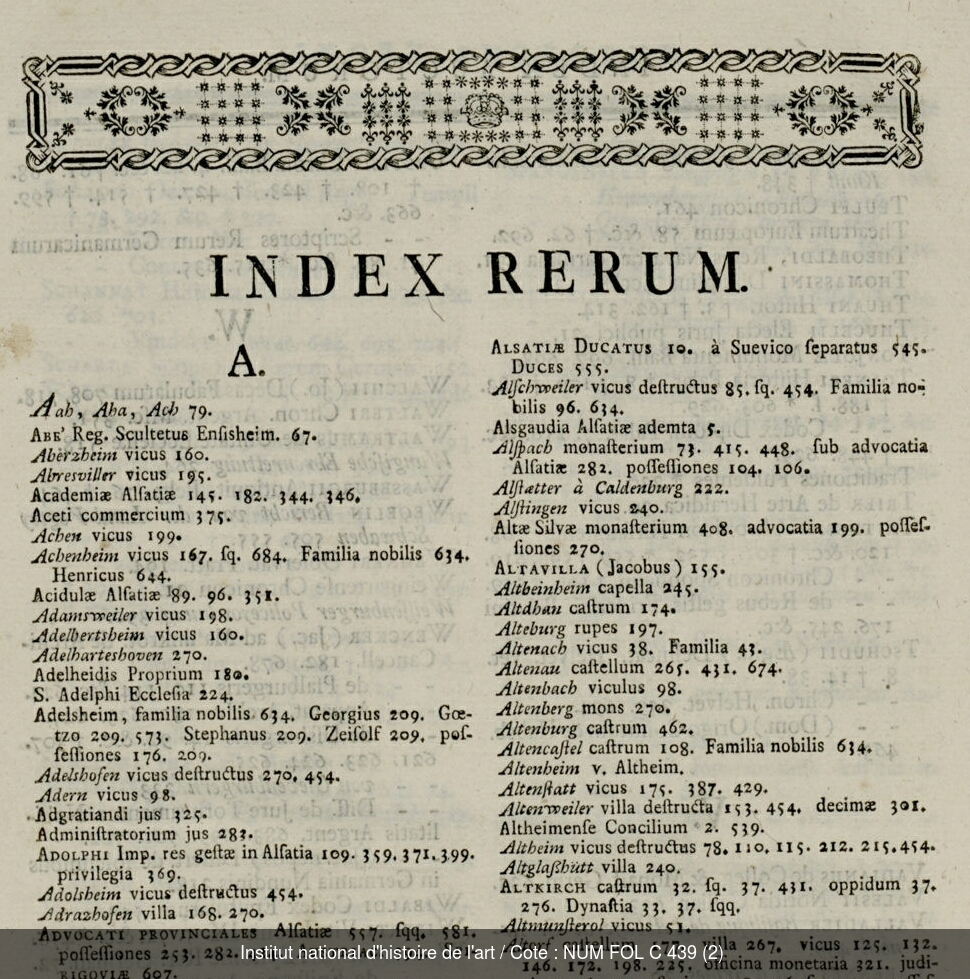
\includegraphics[width=6cm]{images/index_rerum_alsatia.jpg}
		\caption{Index rerum}
	\end{minipage} 
	\medskip
	Extraits des deux index de l'œuvre de \nP{Jean-Daniel}{Schoepflin} [Source: \url{http://bibliotheque-numerique.inha.fr/idurl/1/12532}, p.804 et 813]
\end{figure}

\chapter{\label{annexe_types_interop}Les différents types d'interopérabilité}
\titreEntete{Annexe \thechapter}

\begin{figure}[!h]
	\centering
	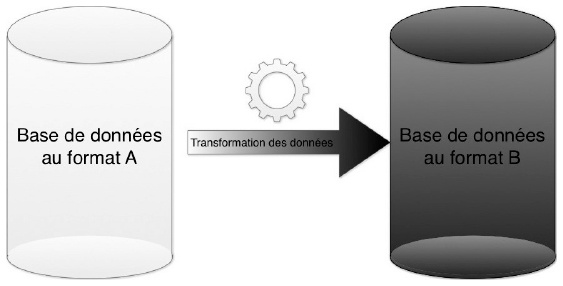
\includegraphics[width=12cm]{images/interop_conversion_copie.jpeg}
	\medskip
	\caption[L'interopérabilité par conversion et copie]{L'interopérabilité par conversion et copie [Source: \cite{bermes_2_2013}]}
\end{figure}

\begin{figure}[!h]
	\centering
	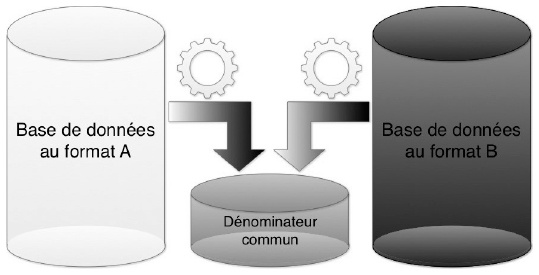
\includegraphics[width=12cm]{images/interop_denom_commun.jpeg}
	\medskip
	\caption[L'interopérabilité par le plus petit dénominateur commun]{L'interopérabilité par le plus petit dénominateur commun [Source: \cite{bermes_2_2013}]}
\end{figure}
	
	\backmatter
	
	
%bibliographie ici dans les normes de l'école
%\printbibliography[title= Bibliographie sélective, prenote=intro]%postnote est aussi possible
%\printbibliography[heading=subbibliography, keyword={semantique}, title={Sémantique}]%biblio sélective pour un mot clé donné

\printindex[referentiels]
\printindex[ina]

	\listoffigures

	\tableofcontents
	
\end{document}